% LaTeX report template 
%

% This is a comment: in LaTeX everything that in a line comes
% after a "%" symbol is treated as comment

\documentclass[11pt, a4paper]{article}
\usepackage{graphicx}
\usepackage{amsmath}
\usepackage{listings}


\title{Assignment 5: The Laplace Equation} % Title

\author{Nithin Babu [EE18B021]} % Author name

\date{\today} % Date for the report
\begin{document}	
\lstset{language=Python}
	
\maketitle % Insert the title, author and date		
  \section*{Abstract}
  The goal of this assignment is the following.
  \begin{itemize}
  \item
  	To solve for currents in a system.
  \item
  	To solve 2-D Laplace equations in an iterative manner.
  \item
	To understand how to vectorize code in python.
  \item
	To plot graphs to understand the 2-D Laplace equation.	
\end{itemize}  	
  
  \section{Introduction}
  This report will discuss about the solver for the currents in a
resistor, the current's dependency on the shape of
the resistor and also which part of the resistor is likely to
get hottest. Here we analyse the currents in a square copper plate to
which a wire is soldered to the middle of it. We find the
currents in the resistor after applying boundary conditions and analyse
the vector plot of current flow and conclude which part of resistor will
become hot.

	\begin{itemize}
    \item
      A wire is soldered to the middle of a copper plate and its voltage is
      held at 1 Volt. One side of the plate is grounded, while the remaining 		  sides are floating. The plate is 1 cm by 1 cm in size.
    \item
      To solve for currents in resistor, we use following equations and
      boundary conditions mentioned below:
    \item
      Conductivity (Differential form of ohm's law)
    \end{itemize}
    
    \begin{equation}
    \vec{J} = \sigma\vec{E}
       \end{equation}
    
    \begin{itemize}
    \item
      Electric field is the gradient of the potential
    \end{itemize}
    
    \begin{equation}
    \vec{E} = -\nabla{\phi}
       \end{equation}
    
    \begin{itemize}
    \item
      Charge Continuity equation is used to conserve the inflow and outflow
      charges
    \end{itemize}
    
    \begin{equation}
    \nabla.\vec{J} = -\frac{\partial \rho}{\partial t}
       \end{equation}
    
    \begin{itemize}
    \item
      Combining the above equations above, we get
    \end{itemize}
    
    \begin{equation}
    \nabla.(-\sigma\nabla\phi) = -\frac{\partial \rho}{\partial t}
       \end{equation}
    
    \begin{itemize}
    \item
      Assuming that our resistor contains a material of constant
      conductivity, the equation becomes
    \end{itemize}
    
    \begin{equation}
    \nabla^{2}\phi = \frac{1}{\sigma}\frac{\partial \rho}{\partial t}
       \end{equation}
    
    \begin{itemize}
    \item
      For DC currents, the right side is zero, and we obtain
    \end{itemize}
    
    \begin{equation}
    \nabla^{2}\phi = 0
       \end{equation}
    
    \begin{itemize}
    \item
      Here we use a 2-D plate so the Numerical solutions in 2D can be easily
      transformed into a difference equation. The equation can be written
      out in
    \end{itemize}
    
    \begin{equation}
    \frac{\partial^{2} \phi}{\partial x^{2}}+ \frac{\partial^{2} \phi}{\partial y^{2}} = 0
     \end{equation}
    
    \begin{equation}
    \frac{\partial \phi}{\partial x}_{(x_i,y_j)} = \frac{\phi(x_{i+1/2},y_j) - \phi(x_{i-1/2},y_j)}{\Delta x}
     \end{equation}
    
    \begin{equation}
    \frac{\partial^{2} \phi}{\partial x^{2}}_{(x_i,y_j)} = \frac{\phi(x_{i+1},y_j) -2\phi(x_i,y_j)+ \phi(x_{i-1},y_j)}{(\Delta x)^{2}}
     \end{equation}
    
    \begin{itemize}
    \item
      Using above equations we get
    \end{itemize}
    
    \begin{equation}
            \phi_{i,j} = \frac{\phi_{i+1,j} + \phi_{i-1,j} + \phi_{i,j+1} + \phi_{i,j-1}}{4} 
    \end{equation}
    
    \begin{itemize}
    \item
      Thus, the potential at any point should be the average of its
      neighbours. This is a very general result and the above calculation is
      just a special case of it. So the solution process is to take each
      point and replace the potential by the average of its neighbours. Keep
      iterating till the solution converges (i.e., the maximum change in
      elements of \(\phi\) which is denoted by \(error_k\) in the code
      ,where 'k' is the no of iteration, is less than some tolerance).
    \item
      At boundaries where the electrode is present, just put the value of
      potential itself. At boundaries where there is no electrode, the
      current should be tangential because charge can't leap out of the
      material into air. Since current is proportional to the Electric
      Field, what this means is the gradient of \(\phi\) should be
      tangential. This is implemented by requiring that \(\phi\) should not
      vary in the normal direction
    \item
      At last we solve for currents in the resistor using all these
      information.
  \end{itemize}

  \section{Potential Array and Initialization}
  

\begin{itemize}
\item
  Define the Parameters, The parameter values taken for my particular code 		  were \(N_x = 25\) and \(N_y = 25\) and number of iterations : 1500
\item
  Allocate the potential array as \(\phi = 0\) .Note that the array
  should have \(N_y\) rows and \(N_x\) columns.
\item
  To find the indices which lie inside the circle of radius 0.35 using
  meshgrid() by equation :
\end{itemize}

\begin{equation}
X ^2 +Y ^2 \leq	 0.35^2
\end{equation}

\begin{itemize}
\item
  Then assign 1 V to those indices.

\end{itemize}

The python code snippet is as shown:
\begin{verbatim}

Nx = 25; 
Ny = 25; 
radius = 8;
Niter = 1500; 
   
phi = zeros((Ny,Nx))
x = linspace(-0.5,0.5,Nx)
y = linspace(-0.5,0.5,Ny)
n = arange(Niter)
X,Y = meshgrid(x,-y)
  
A = (X*X) + (Y*Y)
ii = where(A <= (0.35*0.35))
phi[ii] = 1.0

figure(1)
plot(ii[0]/Nx-0.48,ii[1]/Ny-0.48,'ro',label="V = 1")
title("Initial Potential Contour")
xlim(-0.5,0.5)
ylim(-0.5,0.5)
xlabel(r'$X\rightarrow$')
ylabel(r'$Y\rightarrow$')
grid(True)
legend()  
       \end{verbatim}
       
The plot for the initial potential contour is as shown:
	     \begin{figure}[!tbh]
        \centering
        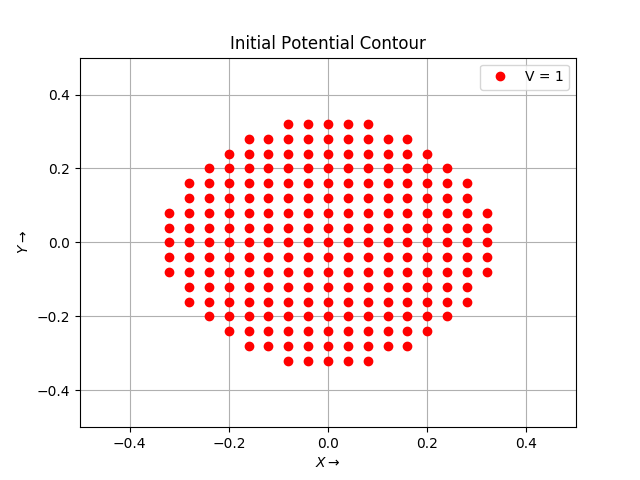
\includegraphics[scale=0.8]{Figure_1.png}  
        \caption{Contour plot of initial potential}
   \end{figure}
 	\newpage
 \section{Potential array updation and iteration}

   \begin{itemize}
   
   \item
    Update the potential \(\phi\) according to Equation below using
     vectorized code
   \end{itemize}
   
   \begin{equation}
           \phi_{i,j} = \frac{\phi_{i+1,j} + \phi_{i-1,j} + \phi_{i,j+1} + \phi_{i,j-1}}{4} 
   \end{equation}
   
   \begin{itemize}
   \item
     To apply Boundary Conditions where there is no electrode, the gradient
     of \(\phi\) should be tangential. This is implemented by Equation
     given below , basically potential should not vary in the normal
     direction so we equate the last but row or column to outermost row or
     column correspondingly when applying boundary conditions for a side of
     plate,implemented using Vectorized code
   \end{itemize}
   
   \begin{equation}
    \frac{\partial \phi}{\partial n} = 0
   \end{equation}
   
   The python code snippet is as shown:

   \begin{verbatim}
    errors = empty((Niter,1))
for k in range(Niter):
    oldphi = phi.copy()
    phi[1:-1,1:-1] = 0.25*(phi[1:-1,0:-2] + phi[1:-1,2:] + phi[0:-2,1:-1] +		                           phi[2:,1:-1])

    phi[1:-1,0] = phi[1:-1,1]
    phi[1:-1,-1] = phi[1:-1,-2]
    phi[0,1:-1] = phi[1,1:-1]
    phi[ii] = 1.0
    errors[k]=(abs(phi-oldphi)).max();
    
         \end{verbatim}
 
 \section{The Error Calculations}  
 \begin{itemize}
 \item
 The error calculated in the last section can be analysed by plotting it against the iteration number.
 \item
 This will give us a much more clearer picture of how the the error varies with respect to the iteration number.
 \end{itemize}
\newpage 
 
The python code snippet for plotting the graphs are as shown:
 \begin{verbatim}
 
# Plotting of error vs iteration in semilog.
figure(2)
semilogy(n,errors)
title("Error versus iteration")
xlabel(r'$Iteration\rightarrow$',size=15)
ylabel(r'$Error\rightarrow$',size=15)
grid(True)

# Plotting of error vs iteration in loglog.
figure(3)
loglog(n,errors)
title("Error versus iteration in a loglog plot")
xlabel(r'$Iteration\rightarrow$',size=15)
ylabel(r'$Error\rightarrow$',size=15)
grid(True)

# Plotting of error vs iteration above 500 in semilog .
figure(4)
semilogy(n[500:],errors[500:])
title("Error versus iteration above 500")
xlabel(r'$Iteration\rightarrow$',size=15)
ylabel(r'$Error\rightarrow$',size=15)
grid(True)

# Plotting of actual and expected error (above 500 iterations) in semilog.
figure(5)
semilogy(n[500:],errors[500:],label="Actual")
semilogy(n[500:],a_500*exp(b_500*n[500:]),label="Expected")
title("Expected versus actual error (>500 iterations)")
xlabel(r'$Iteration\rightarrow$',size=15)
ylabel(r'$Error\rightarrow$',size=15)
grid(True)
legend()
\end{verbatim}       
\newpage
The respective error plots are as shown:

    
     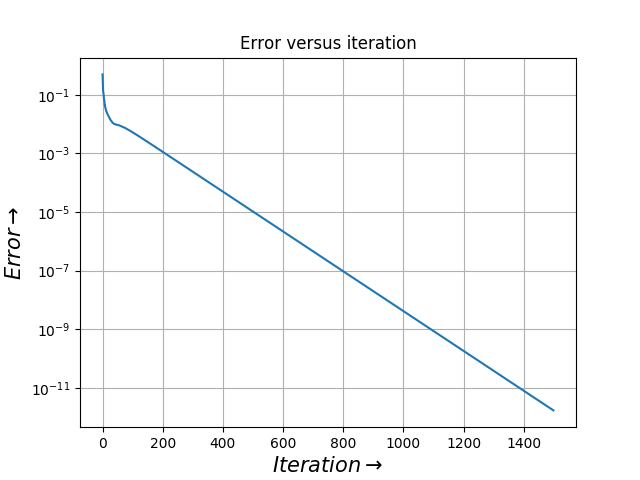
\includegraphics[scale=0.8]{Figure_2.png} 
     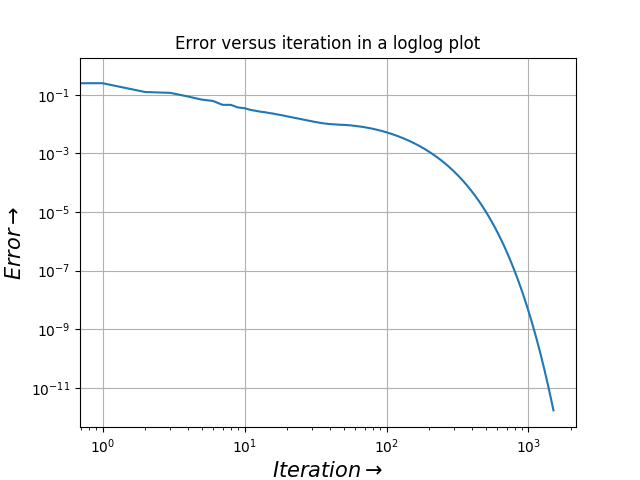
\includegraphics[scale=0.8]{Figure_3.png}  
     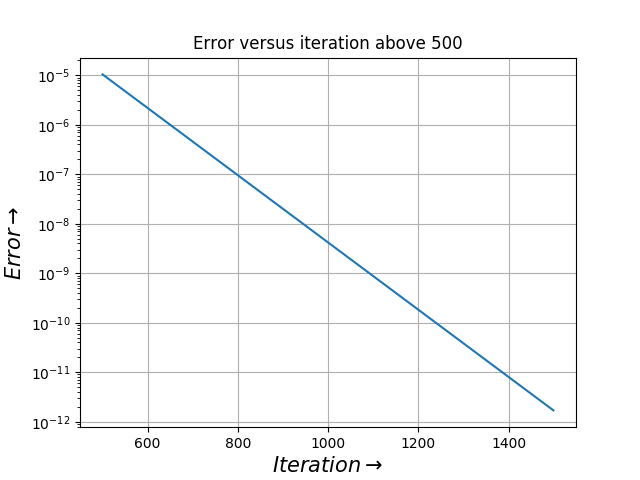
\includegraphics[scale=0.8]{Figure_4.png}  


\subsubsection*{Extracting the exponential}

\begin{itemize}
\item
  We can find the fit using Least squares for all iterations
  separately and compare them.
\item
  As we know that error follows \(Ae^{Bx}\) at large iterations, we use
  equation given below to fit the errors using least squares.
\end{itemize}

\begin{equation}
    logy = logA + Bx
\end{equation}

\begin{itemize}
\item
  We can find the constants of the error function obtained for the two cases
  using lstsq and compare them.
\end{itemize}

The python code snippet to extract the exponent is as follows:

   \begin{verbatim}
   
c_approx_500 = 
lstsq(c_[ones(Niter-500),arange(500,Niter)],log(errors[500:]),rcond=None)  
a_500,b_500 = exp(c_approx_500[0][0]),c_approx_500[0][1]

c_approx = lstsq(c_[ones(Niter),arange(Niter)],log(errors),rcond=None)
a, b = exp(c_approx[0][0]), c_approx[0][1] 
\end{verbatim}
\newpage
The plots comparing both the errors are as shown:

\begin{figure}[!tbh]
 \centering
 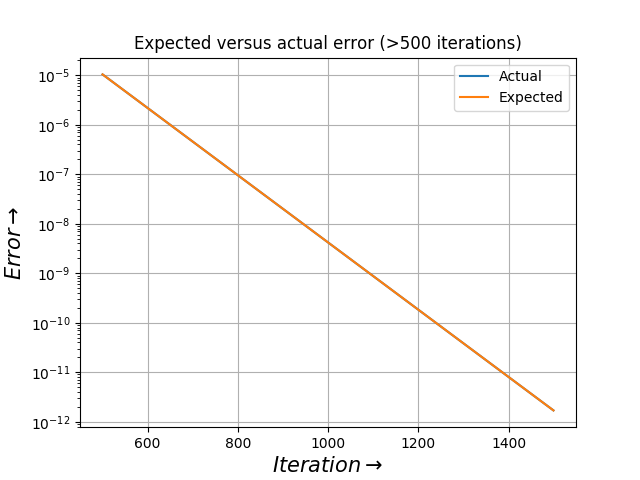
\includegraphics[scale=0.7]{Figure_5.png}  
 \caption{Expected versus actual error (above 500 iterations)}
\end{figure}

\begin{figure}[!tbh]
 \centering
 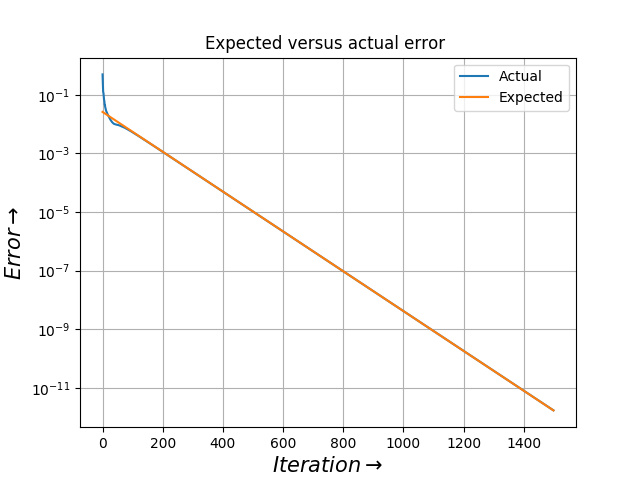
\includegraphics[scale=0.7]{Figure_6.png}  
 \caption{Expected versus actual error}
\end{figure}

\newpage
Upon execution of the code, we can observe that 
\begin{itemize}
\item
$ A_{500} = 0.02604399$ and $B_{500} = -0.01564807 $ 

\item
$A = 0.02621557$ and $B = -0.01565526$

\end{itemize}


\section{Surface and Contour Plot of Potential}

We can analyse the potential variations by plotting it as a surface and contour plot. The following python code explains it. 
\begin{verbatim}
 figure(7)
 contourf(X,Y,phi)
 plot(ii[0]/Nx-0.48,ii[1]/Ny-0.48,'ro',label="V = 1")
 title("Contour plot of potential")
 xlabel(r'$X\rightarrow$')
 ylabel(r'$Y\rightarrow$')
 colorbar()
 grid(True)
 legend()
 
 fig1=figure(8)
 ax=p3.Axes3D(fig1) 
 title("The 3-D surface plot of the potential")
 xlabel(r'$X\rightarrow$')
 ylabel(r'$Y\rightarrow$')
 surf = ax.plot_surface(X, Y, phi, rstride=1, cstride=1, cmap=cm.jet)
 fig1.colorbar(surf)
 
 show()
  \end{verbatim}
\newpage
The surface and contour plots are as shown below:

\begin{figure}[tbh]
 \centering
 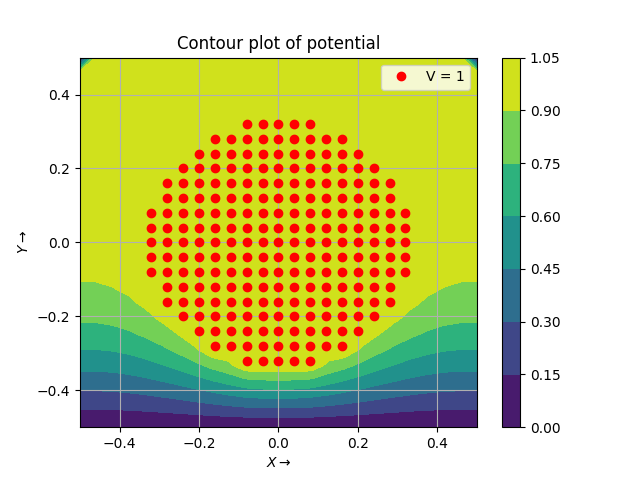
\includegraphics[scale=0.7]{Figure_7.png}  
 \caption{Contour plot of potential}
\end{figure}

\begin{figure}[!tbh]
 \centering
 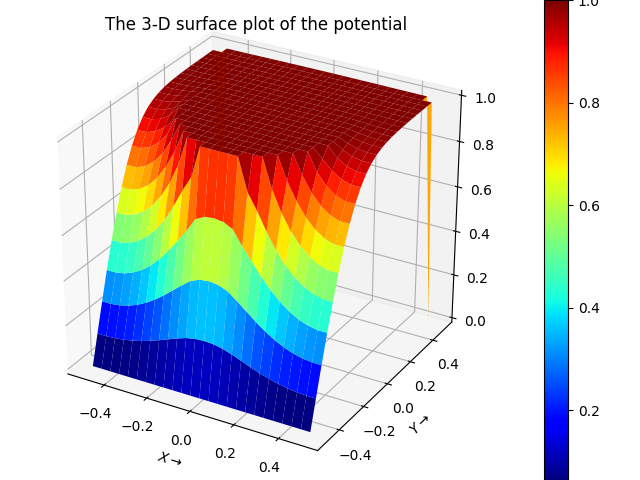
\includegraphics[scale=0.7]{Figure_8.png}  
 \caption{3-D Surface potential plot of potential}
\end{figure}
\newpage
\newpage

\section{Vector Plot of Currents}

\begin{itemize}
\item
  We can obtain the currents by computing the gradient.
\item
  The actual value of \(\sigma\) does not matter to the shape of the
  current profile, so we set it to unity. Our equations are
\end{itemize}

\begin{equation}
    J_x = -\frac{\partial \phi}{\partial x} 
  \end{equation}

\begin{equation}
    J_y = -\frac{\partial \phi}{\partial y} 
  \end{equation}

\begin{itemize}
\item
  To program this we use these equations as follows:
\end{itemize}

\begin{equation}
        J_{x,ij} = \frac{1}{2}(\phi_{i,j-1} - \phi_{i,j+1}) 
    \end{equation}

\begin{equation}
        J_{y,ij} = \frac{1}{2}(\phi_{i-1,j} - \phi_{i+1,j}) 
    \end{equation}
  
The python code snippet for calculating the the current densities and plotting them are as follows:
   
  
\begin{verbatim}

 Jx = zeros((Ny, Nx))
 Jy = zeros((Ny, Nx))
 Jx[1:-1, 1:-1] = 0.5*(phi[1:-1, 0:-2] - phi[1:-1, 2:])
 Jy[1:-1, 1:-1] = 0.5*(phi[2:, 1:-1] - phi[0:-2, 1:-1])
 
 figure(0)
 quiver(X,Y,Jx,Jy)
 plot(ii[0]/Nx-0.48,ii[1]/Ny-0.48,'ro')
 title("The vector plot of the current flow")
 xlabel(r'$X\rightarrow$')
 ylabel(r'$Y\rightarrow$')
  \end{verbatim}
  \newpage
The vector plot of the current flow along with the potential is as shown below:

  \begin{figure}[!tbh]
   \centering
   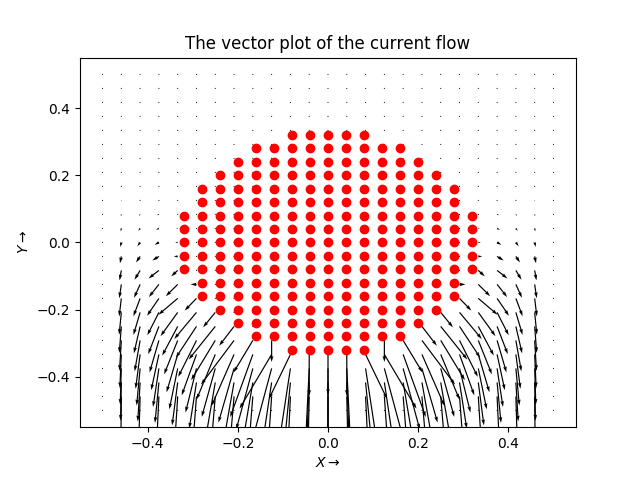
\includegraphics[scale=0.8]{Figure_0.png}  
   \caption{Vector plot of current flow}
  \end{figure}
  

  \begin{itemize}
  \item
    So as we noted that the potential gradient was higher in down region
    of the plate, and we know that Electric field is the gradient of the
    potential as given below
  \end{itemize}
  
  \begin{equation}
  \vec{E} = -\nabla{\phi}
     \end{equation}
  
  \begin{itemize}
  \item
    So \(\vec{E}\) is larger where there is potential gradient is high and
    is inverted since it is negative of the gradient!, So it is higher in
    down region which is closer to bottom plate which is grounded
  \item
    And we know that
  \end{itemize}
  
  \begin{equation}
  \vec{J} = \sigma\vec{E}
     \end{equation}
  
  \begin{itemize}
  \item
    So \(\vec{J}\) is higher and perpendicular to equipotential electrode
    region i.e "Red dotted region" so the current is larger in down part
    of the plate and perpendicular to the red dotted electrode region
    since \(I\) = \(\vec{J}.\vec{A}\)
  \item
   	This is the reason most of the current flows from electrode to the
    bottom plate which is grounded because of higher potential gradient.
  \item
    And there is almost zero current in upper part of the plate since
    there is not much potential gradient as we observed from the surface
    and contour plot of the potential \(\phi\)
  \end{itemize}
  
    
  
    
      
  \section{Conclusion :}
  
  \begin{itemize}
  \item
    To conclude , most of the current is in the narrow region at the
    bottom. So this region will get strongly heated.
  \item
    Since there is almost no current in the upper region of plate, the
    bottom part of the plate gets hotter and temperature increases in down
    region of the plate.
  \item
    And we know that heat generated is from \(\vec{J}.\vec{E}\) (ohmic
    loss) so since \(\vec{J}\) and \(\vec{E}\) are higher in the bottom
    region of the plate, there will more heat generation and temperature
    rise will be present.
  \item
    So overall we looked the modelling of the currents in resistor in this
    report ,and we observe that the best method to solve this is to
    increase \(N_x\) and \(N_y\) to very high values (100 or \(\geq\)
    100) and increase the number of iterations too, so that we get accurate
    answers i.e currents in the resistor.
  \item
    But the trade off is this method of solving is very slow even though we
    use vectorized code because the decrease in errors is very slow w.r.t
    no of iterations.
  \end{itemize}
  \end{document}